\documentclass{if-beamer}

% --------------------------------------------------- %
%                  Presentation info	              %
% --------------------------------------------------- %
\title[Lecture 15]{Lecture 15}
\subtitle{Optimization: Coding the Golden Section Search Method}
\author{Ashley Gannon}
\date{ISC3313 Fall 2021}
\logo{

\includegraphics[scale=0.08]{figures/FSULogo.png}
}
\subject{Presentation subject}

% --------------------------------------------------- %
%                    Title + Schedule                 %
% --------------------------------------------------- %
\begin{document}

\begin{frame}
  \titlepage
\end{frame}
% --------------------------------------------------- %
%                      Presentation                   %
% --------------------------------------------------- %
\section{Wrapping up the Golden-Section Search Method}

\begin{frame}
\frametitle{Golden-Section Search Method Pseudocode Example}

\texttt{define/declare phi}\\
\texttt{declare tol, x1, x2, d, xopt}\\
\texttt{declare/define error}\\\vspace{10pt}
\texttt{d = (phi -1)(xu-xl)}\\
\texttt{x1 = xl+d;}\\
\texttt{x2 = xu-d;}\\\vspace{10pt}
\texttt{while error>tol}\\
\texttt{\qquad if f(x1)<f(x2)}\\
\texttt{\qquad \qquad xl = x2;}\\
\texttt{\qquad \qquad x2 = x1;}\\
\texttt{\qquad \qquad d = (phi-1)(xu-xl);}\\
\texttt{\qquad \qquad x1 = xl + d;}\\
\texttt{\qquad \qquad xopt = x1;}\\
\texttt{\qquad else}\\
\texttt{\qquad \qquad xu = x1;}\\
\texttt{\qquad \qquad x1 = x2;}\\
\texttt{\qquad \qquad d = (phi-1)(xu-xl);}\\
\texttt{\qquad \qquad x2 = xu-d;}\\
\texttt{\qquad \qquad xopt = x2;}\\
\texttt{\qquad error = (2-phi)*abs((xu-xl)/xopt);} \\	

\end{frame}

\begin{frame}
	\frametitle{Let's code it!}
	We are going to write this function and apply it to
	$$f(x) = \frac{x^2}{10}-2sin(x)$$
	With an initial $x_l =0$, $x_u =4$. Remembering our plot:
	\begin{figure}
		\centering
		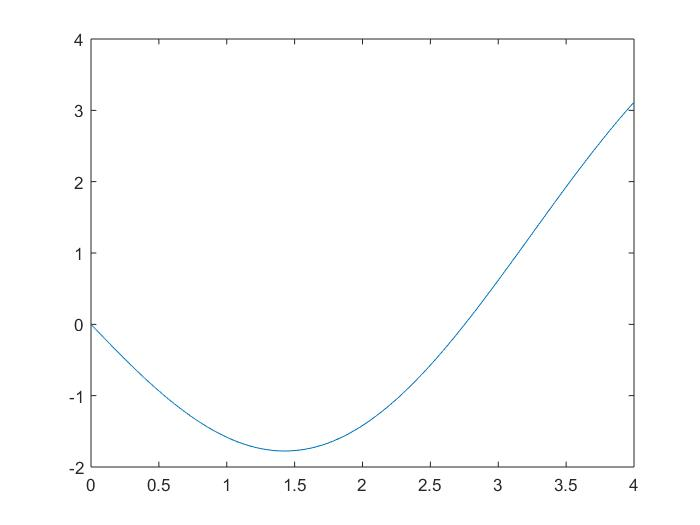
\includegraphics[width=.6\textwidth]{figures/plot}
	\end{figure}
	When you have finished your code, post it in the \textbf{Golden-Section Search Code} discussion board.
\end{frame}


\end{document}
